%! Author = domore
%! Date = 8/11/21

% Preamble
\documentclass[11pt]{article}

% Packages
\usepackage{amsmath}
\usepackage{graphicx}
\usepackage{cleveref}
\usepackage[margin=1.1in]{geometry}
\usepackage{python}
\usepackage{pythontex}
%pdflatex -aux-directory=/home/domore/PycharmProjects/ds_project-1/document_files/aux -output-directory=/home/domore/PycharmProjects/ds_project-1 main_document.tex
%python document_files/pythontex/pythontex3.py document_files/main_document.tex
%pdflatex -aux-directory=/home/domore/PycharmProjects/ds_project-1/document_files/aux -output-directory=/home/domore/PycharmProjects/ds_project-1 main_document.tex
\usepackage[framemethod=TikZ]{mdframed}

% for future projects
% \usepackage[usefamily=juliacon]{pythontex}

% Document
\begin{document}

\part[wine]{Project 1: Wine Quality}


\begin{pyconsole}[][frame=single]
import pandas as pd
import os

# Referencing folders and data names
path = os.getcwd()
# We have to re-structure the path since we are in LaTeX
path = os.path.abspath(os.path.join(path, os.pardir))
file_name = 'winequality-red.csv'
path_file = f'{path}/code_python/project1_wine/data/{file_name}'
# We load the data and present an overview
wine_data = pd.read_csv(path_file)
wine_data.info()
\end{pyconsole}

We first check that the correlation structure amongst the variables (see \cref{fig:wine_heatmap}),
including the quality of the wine.
This should give us a general idea of how and if the variables are related to one another.

\begin{pycode}
print('Hello, World')
\end{pycode}

\begin{figure}[h!]
    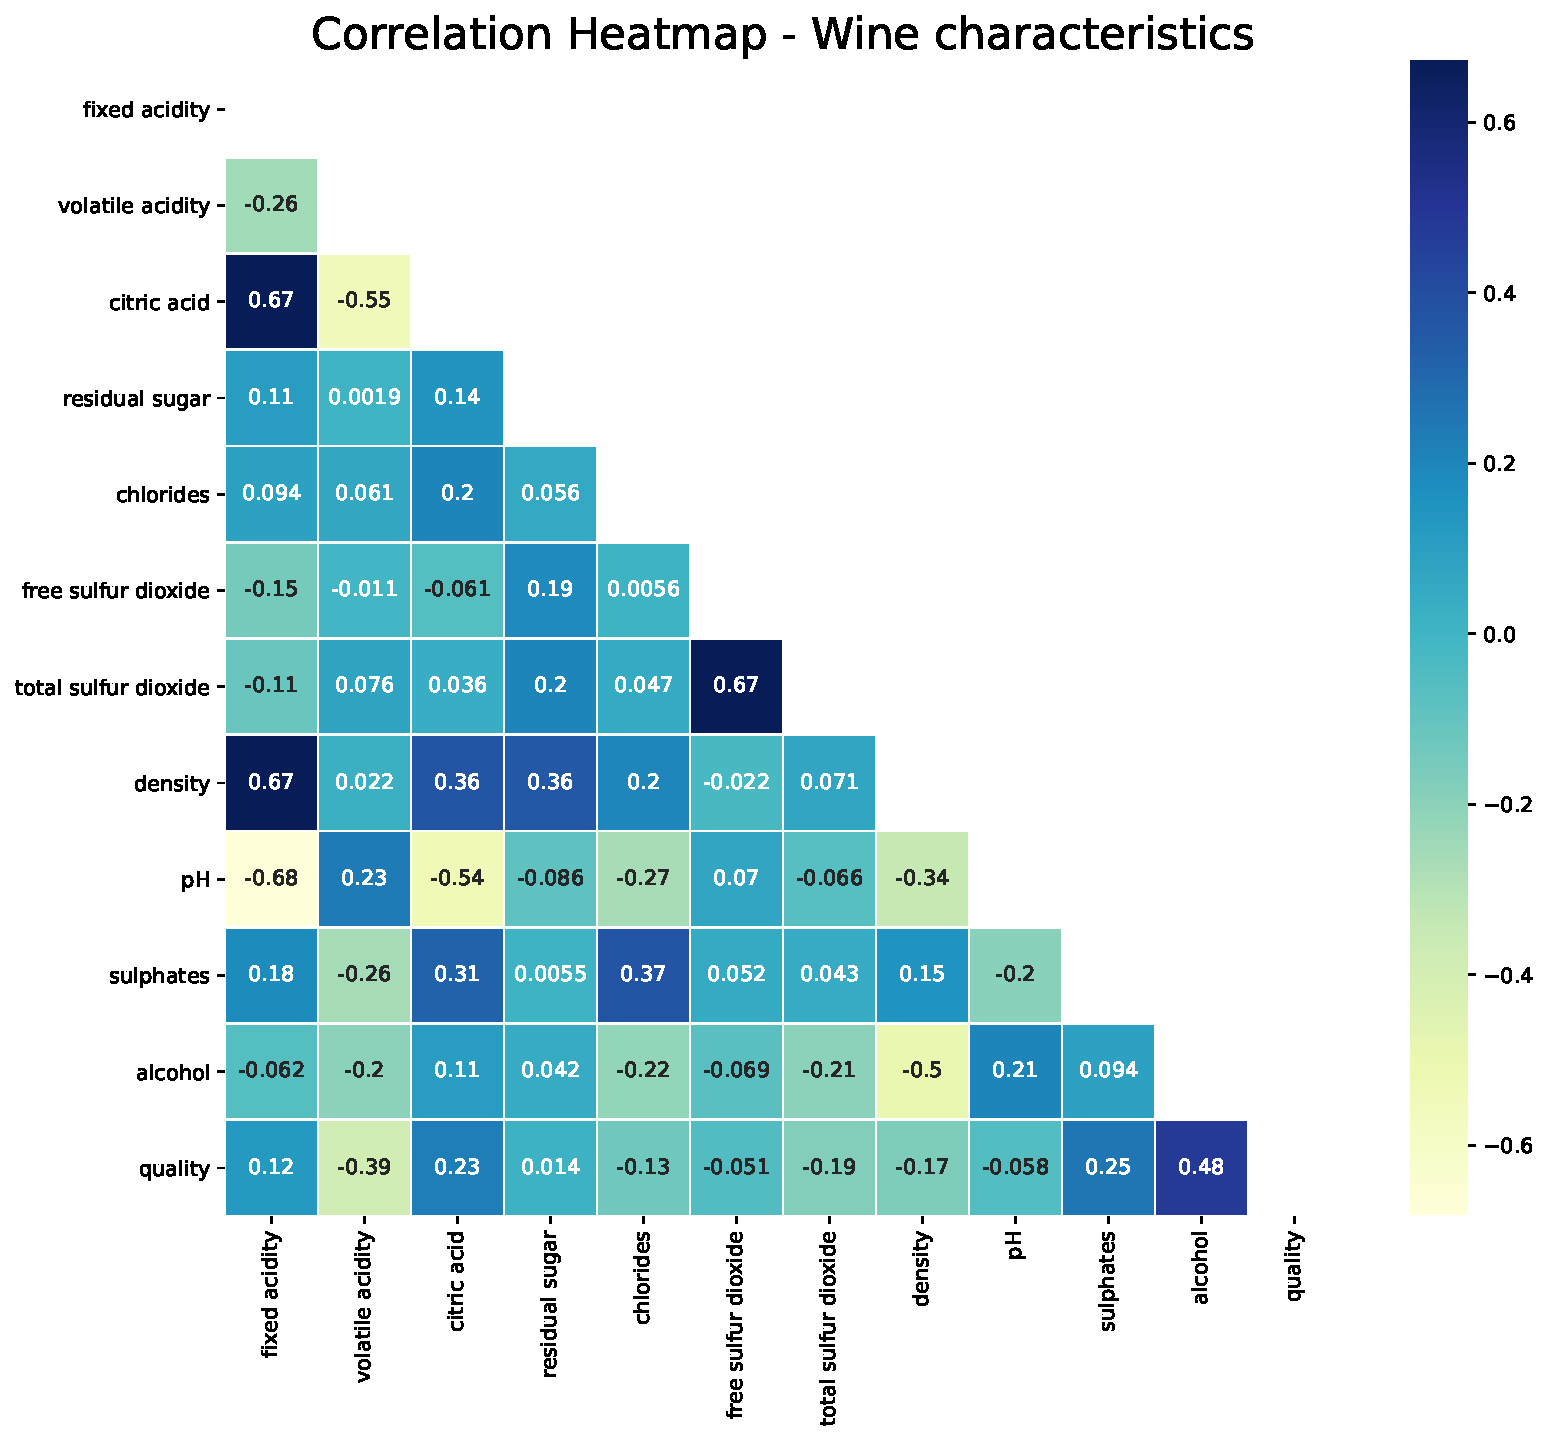
\includegraphics[width=0.9\textwidth]{figs/wine_heatmap}
    \caption{Correlation structure of wine characteristics.}
    \label{fig:wine_heatmap}
\end{figure}

There are a few things we could appreciate to check whether the data we are looking relates somehow
to our prior knowledge about the topic.
This prior knowledge might help us identify certain links, that might not be obvious if the data were not labeled.

At first glance, one can note that \emph{fixed acidity} is strongly correlated (negatively) to the \emph{pH},
although their correlation is not \emph{1}.
Additionally, we can see that \emph{alcohol} correlates negatively with the \emph{density} of the wine.
This makes sense, given that the wine is a solution of different solutes, those in all likelihood are ``heavier''
than the alcohol solute.
Hence, the more the alcohol content increases in the wine, the less dense it becomes.
\vspace{2pt}
Another visual analysis we could perform is to look at the KDEs (Kernel Density Estimates).
These we could imagine as a cross-sectional cut in a bi-variate probability distribution.
\Cref{fig:wine_kdes} shows us that even though the wines in the sample range from quality 3 to 8
(see subplot in row 3, column 4), it would seem that there are mostly 4 important groups.
The earlier stated fact, ad priori, gives us an interesting thing we should have in mind when trying
to fit any kind of model.
I.e., the tails of the quality (grades 3 and 8) will be underrepresented, then most model we could think
of fitting will have trouble predicting a grade close to 3 and 8 and beyond (to each direction).

\begin{figure}[h!]
    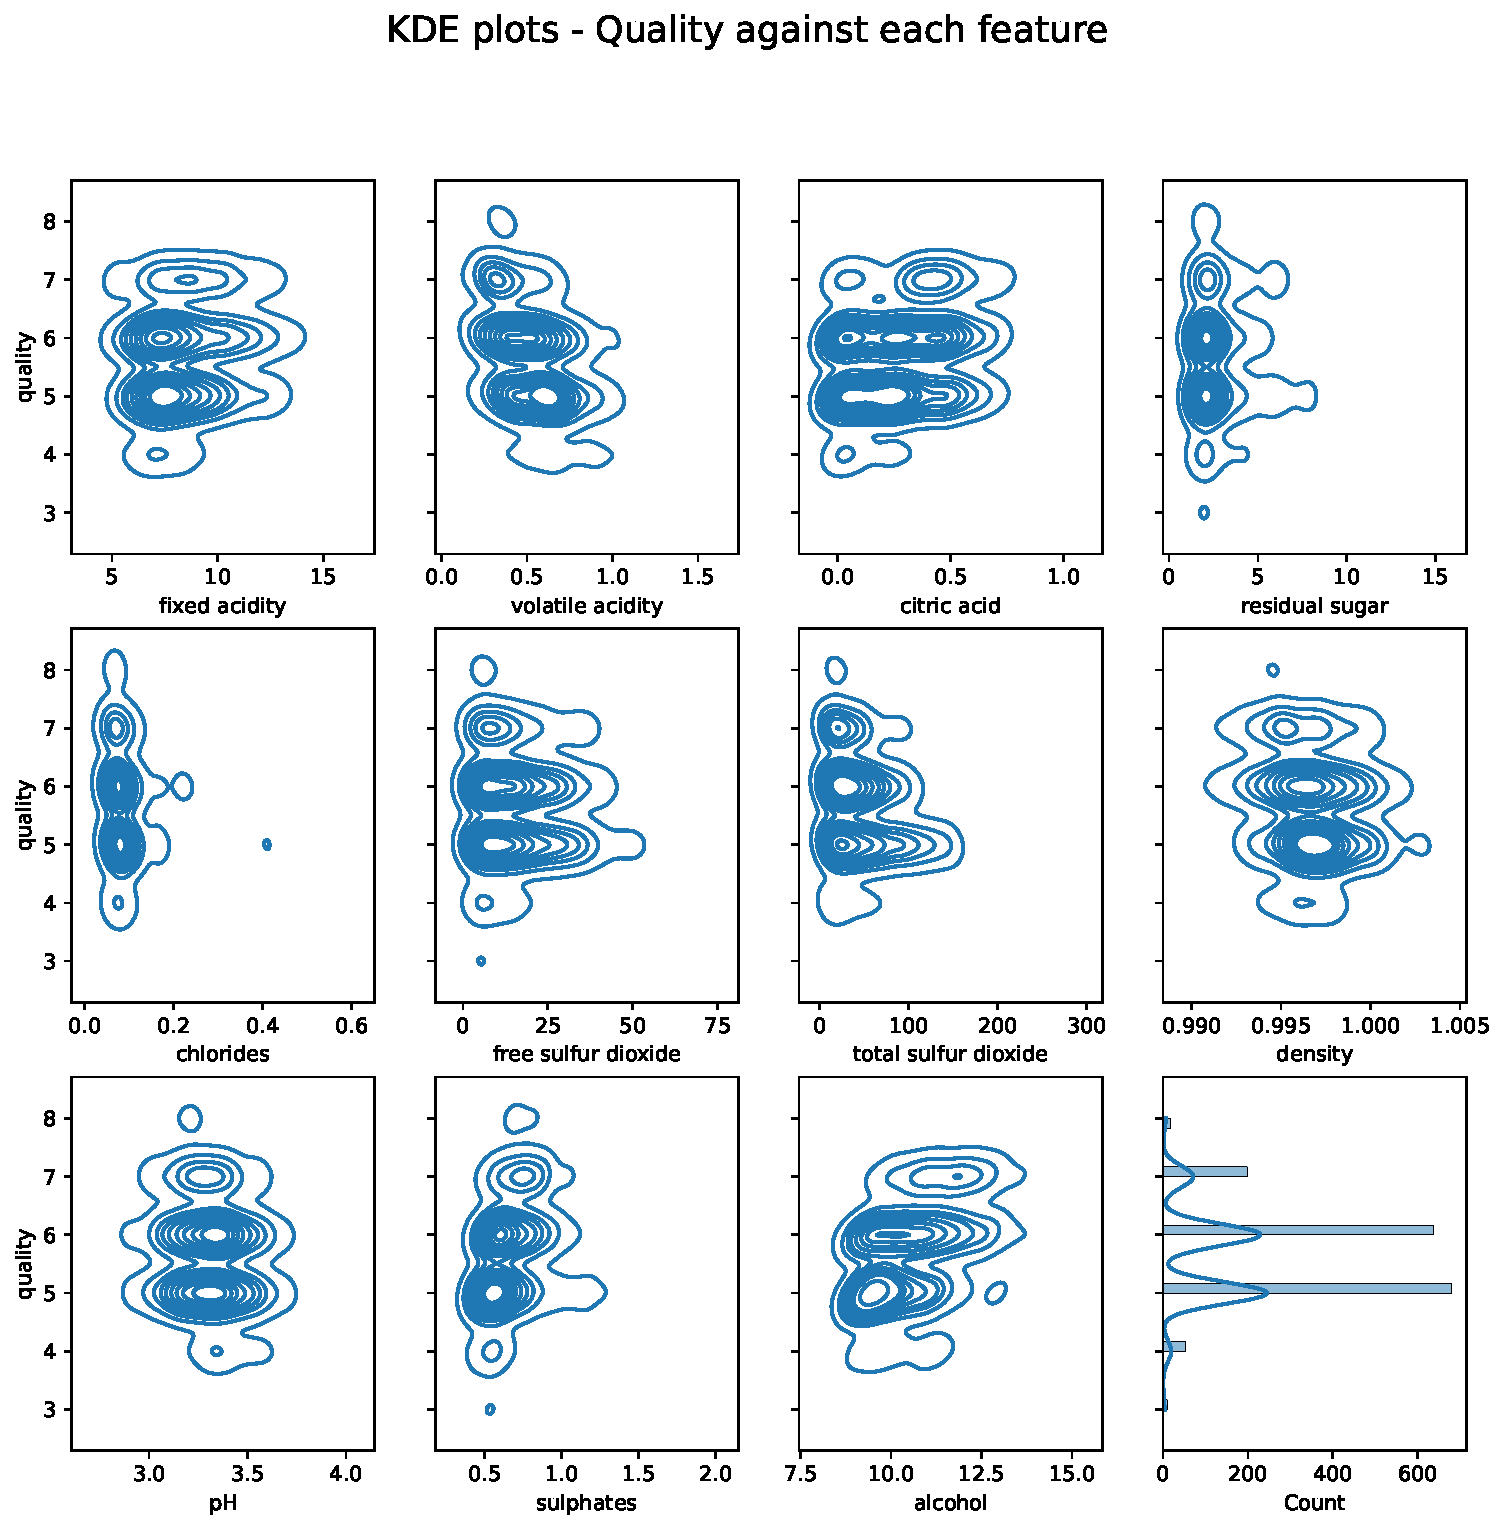
\includegraphics[width=0.9\textwidth]{figs/wine_kde}
    \caption{KDEs for wine features.}
    \label{fig:wine_kdes}
\end{figure}

\newpage
\part[food]{Project 2: Food Preferences}


\newpage
\part[stores]{Project 3: Store Sales}



\end{document}